\section*{Experimentation}

In this experimental part we are going to both study the numerical stability and limit of the method and compare to existing non-trivial benchmark problems. Here, supervised learning is targeted since it is a direct way to evaluate the method efficiency and robustness. Let us remember that we do not evaluate learning performances here, only the way me can adjust recurrent network weights. We only study the estimation convergence here, not the learning properties (such as generalization, capacity, ...).

\subsection*{Software implementation}

In order to provide so called reproducible science \cite{topalidou_long_2015}, the code is implemented as a very simple, highly modular, fully documented, open source, object oriented, easily forkable, self contained, middle-ware, \href{nowhere:not-yet-on-line}{available here}. A minimal set of standard mechanisms (random number generation, histogram estimation, linear system resolution, system calls) is used. The main part of the implementation hierarchy is show in Fig.~\ref{class-hierarchy}. 

\begin{figure}[!ht]
  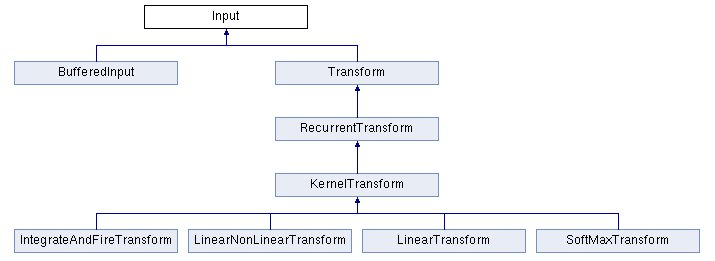
\includegraphics[width=0.8\textwidth]{img/class-hierarchy}
  \caption{A view of the class-hierarchy: A {\tt Input} simply provides a $x_n(t), n \in \{0, N\{, t \in \{0, T\{$ values, while a {\tt Transform} provides such values given another {\tt Input}, while other objects defined here derive from such an oversimple abstract class.}
  \label{class-hierarchy}
\end{figure}

For run-time performances and inter-operability with different programming languages a {\tt C/C++} implementation (with the compilation scripts) is proposed, the wrapping to other programming languages (e.g., {\tt Python}) being straightforward, using e.g. {\tt swig}. 

The first experimental verification was that it was very simple to define the main unit structures reviewed in section~\ref{generality} from {\tt KernelTransform} as claimed in the paper.

\subsection*{Numerical stability and limit of the method}

Regarding this first issue, as being in a deterministic context, we are going to rely on a reverse engineering setup: An input/output learning sequence is going to be generated by a input/output root network of $\bar{N}$ units and another learning network with random initialization is going to re-estimate a transform. This guaranty the existence of an exact solution. 

How revelant is it to use such a reverse engineering setup ? On one hand, surprisingly enough perhaps, such networks (at least deep networks \cite{Zhang2016Understanding}) behave with the same order of magnitude of performances, the input being either ``meaningful'' in the sense it represents data with a semantic or not. We thus can expect simple random input/output tests to be relevant to more specific application. On the other hand we are going to develop in the next section how several ``challenging'' tests are in fact highly dependent on the chosen architecture, with often trivial solution, as soon as the hidden architecture is well chosen.

Considering random input/output with some statistics, in most of the cases, they are several solutions (e.g. up to a permutation of the units, or some linear combination in a linear case, ...). We consider a root network of $\bar{N}$ units for a sequence of time $T$, for a $M=1$ scalar input, considering either L (for linear), LNL or AIF units, with random weights (drawn from a Gaussian distribution with $0$ mean and $\sigma \simeq 1/N$ standard deviation, which is know to guaranty a stable non-trivial dynamic). Only the unit of index $n=0$ is considered as output units, i.e., $N_0 = 1$, the $N-1$ remainder units activity being hidden to the estimation.

In this determistic case, we observe two main parameters the final precision criterion value ${\cal L}$ and the number of steps to convergence $S$. 

A step further, we also study exact solution or approximation, we are going to consider learning network with $N \leq \bar{N}$ units, i.e. networks that do not generate the exact solution. We already know that as soon as the dynamic is sufficiently rich, even small errors accumulates and the solution exponentially diverges from the exact one. In such a case the question is wether the input/output statistics also diverges. We thus have to compare the KL-divergence between the desired and obtained output given the input. The fact we chose $N_0 = 1$ makes this estimation tracktable since it is a 1D distribution. OUI MAIS JUSTE HISTOGRAMME QUID DE LA DEPENDENCE EN i(t-R) ?

\subsection*{Comparison with existing estimation problems}

Let us now discuss how our validation method compares with usual benchmark for recurrent network estimation.
